\documentclass[
]{thesis-ekf}
\usepackage[T1]{fontenc}
\PassOptionsToPackage{defaults=hu-min}{magyar.ldf}
\usepackage[magyar]{babel}
\usepackage{mathtools,amssymb,amsthm,pdfpages}
\usepackage{graphicx, url}
\usepackage{listings,xcolor,caption,upquote}
\lstloadlanguages{JavaScript}
\footnotestyle{rule=fourth}

\newtheorem{tetel}{Tétel}[chapter]
\theoremstyle{definition}
\newtheorem{definicio}[tetel]{Definíció}
\theoremstyle{remark}
\newtheorem{megjegyzes}[tetel]{Megjegyzés}

\lstset{
	inputencoding=utf8,
	basicstyle=\footnotesize\ttfamily,
	columns=fullflexible,
	numbers=left,
	breaklines,
	postbreak=\hbox{$\mathcolor{red}{\hookrightarrow}$\ },
	xleftmargin=2cm,
	xrightmargin=2cm,
	frame=single,
	literate={ó}{\'{o}}1
	{á}{\'{a}}1,
}

\lstdefinestyle{myjavascript}{
	language=JavaScript,
	backgroundcolor=\color{cyan!10},
	keywordstyle=\color{blue},
	commentstyle=\itshape\color{teal},
	identifierstyle=\color{black},
	stringstyle=\color{red},
}


\renewcommand{\lstlistingname}{kód}

\begin{document}
	
	\institute{Matematikai és Informatikai Intézet}
	\title{Személyi igazolványok digitális tárolása}
	\author{Kovács Gábor\\programtervező informatikus}
	\supervisor{Dr. Kovásznai Gergely\\Tanszékvezető, egyetemi docens}
	\city{Eger}
	\date{2025}
	\maketitle
	
	\tableofcontents
	
	\chapter*{Bevezetés}
	
	\chapter{Személyazonosítás fejlődése és digitalizációja}
	
	\section{A személyi igazolványok története}
	A személyazonosítás igénye évezredekre nyúlik vissza, hiszen a társadalmak mindig is szerették volna hiteles módon azonosítani tagjaikat. Az ókori birodalmakban pecsétes levelek és különböző azonosító jegyek szolgáltak erre a célra. A középkorban a nemesi kiváltságokat vagy állampolgárságot igazoló dokumentumokat használtak, például a pápai bullákat vagy a királyi rendeleteket.
	A modern értelemben vett személyi igazolványok a 19. és 20. században terjedtek el, amikor az államok egyre inkább szükségét érezték annak, hogy állampolgáraikat hivatalos dokumentumokkal azonosítsák. Magyarországon az első személyi igazolványokat a második világháború után vezették be, és azóta számos változáson mentek keresztül, mind biztonsági, mind technológiai szempontból.
	
	\section{A digitális azonosítás megjelenése}
	A 21. században a digitális technológia fejlődésével a személyazonosítás egyre inkább az elektronikus rendszerekre helyeződött át. Az internet elterjedésével növekedett az igény a biztonságos online azonosításra, amely a hagyományos személyi igazolványok digitális megfelelőit hívta életre.
	
	Számos országban bevezették az elektronikus személyi igazolványokat (eID), amelyek beépített chippel rendelkeznek, és különböző biometrikus adatokat is tárolhatnak, mint ujjlenyomat vagy arcfelismerési információ. Ezek az azonosítási módszerek jelentősen javítják a biztonságot és megkönnyítik az online szolgáltatásokhoz való hozzáférést.
	
	\section{A mobiltechnológia és az azonosítás}
	Az okostelefonok és a mobilalkalmazások terjedésével az azonosítás folyamata tovább egyszerűsödött. A felhasználók ma már egyetlen kattintással vagy biometrikus azonosítással (pl. Face ID, ujjlenyomat-olvasó) hitelesíthetik magukat különböző szolgáltatásokhoz.
	A mobiltechnológia lehetővé tette a digitális személyazonosítás gyorsabb, kényelmesebb és biztonságosabb formáit. A blockchain alapú azonosítási rendszerek pedig tovább fokozzák az adatok védelmét, lehetőséget adva a felhasználóknak, hogy nagyobb kontrollt gyakoroljanak személyes adataik felett.
	
	\section{A digitalizáció jövője a személyazonosításban}
	A jövőben a személyazonosítás módszerei tovább fejlődnek, egyre inkább az automatizált és AI-alapú rendszerek irányába. Az arcfelismerés, a hangalapú azonosítás és a viselkedéselemzés egyre népszerűbbé válik.
	
	A digitális személyazonosítás előnye, hogy gyorsabb és hatékonyabb az offline módszereknél, ugyanakkor komoly adatbiztonsági kihívásokat is felvet. A jövő fejlesztései során kulcsfontosságú lesz a magánszféra védelme és az etikus adatkezelés biztosítása.
	
	\chapter{Digitális személyi igazolványok: Előnyök és kihívások}
	A digitális személyi igazolványok (e-személyik) az állampolgárok azonosításának egyre népszerűbb eszközei világszerte. Ezek az okmányok nemcsak a hagyományos, fizikai igazolványok elektronikus megfelelői, hanem további funkciókkal is rendelkezhetnek, például online hitelesítésre, elektronikus aláírásra vagy egyes állami és magánszolgáltatások elérésére.
	
	Bár a digitális személyazonosítás rengeteg előnyt kínál, számos kihívás is társul hozzá, amelyek megoldása kulcsfontosságú a széleskörű elterjedéshez.
	\section{Előnyök}
	\subsection{Kényelem és gyorsaság}
	A digitális személyi igazolványok lehetővé teszik az azonosítás és hitelesítés gyors és kényelmes módját. Az állampolgárok anélkül igazolhatják magukat, hogy fizikai okmányt kellene magukkal hordaniuk, hiszen az azonosító adatok tárolhatók egy mobiltelefonon vagy egy biztonságos szerveren.
	
	Például egy e-személyi igazolvány segítségével egy banki ügyintézés vagy egy online regisztráció néhány kattintással elvégezhető, míg a hagyományos személyazonosítás esetében papírokat kell kitölteni, aláírni és személyesen bemutatni.
	\subsection{Biztonság és hitelesség}
	A digitális személyi igazolványok a legmodernebb titkosítási technológiákat alkalmazzák, így nehezebben hamisíthatók, mint a hagyományos plasztikkártyák. Egy jól megtervezett digitális rendszerben az adatok ellenőrzése és tárolása szigorú biztonsági szabványok szerint történik, csökkentve az illetéktelen hozzáférés vagy visszaélés esélyét.
	
	Biometrikus azonosítókkal (például arcfelismerés vagy ujjlenyomat) kombinálva az e-személyik még biztonságosabbá válhatnak, hiszen a felhasználó azonosítása egyértelmű és nehezen másolható.
	\subsection{Fenntarthatóság és költséghatékonyság}
	A digitális személyi igazolványok hozzájárulhatnak a papíralapú ügyintézés csökkentéséhez, ami nemcsak a környezetvédelmet szolgálja, hanem a közigazgatási rendszerek hatékonyságát is növeli. A kevesebb nyomtatás, postázás és manuális adatfeldolgozás hosszú távon jelentős költségmegtakarítást eredményezhet az állam és a vállalatok számára is.
	\section{Kihívások}
	\subsection{Adatvédelem és biztonsági kockázatok}
	A digitális személyazonosító rendszerek egyik legnagyobb kihívása az adatbiztonság. Mivel ezek az igazolványok személyes adatokat tartalmaznak, kiemelt célpontjai lehetnek kibertámadásoknak és adatlopásoknak. Egy esetleges rendszerfeltörés vagy adatvédelmi incidens súlyos következményekkel járhat az érintettek számára.
	
	Ennek elkerülése érdekében olyan technológiákat kell alkalmazni, mint a többfaktoros hitelesítés, az adatok titkosítása és a decentralizált adattárolás. Az adatvédelmi jogszabályok (például az EU GDPR rendelete) is szigorúan szabályozzák, hogy a digitális személyi igazolványokhoz kapcsolódó információkat hogyan lehet kezelni és tárolni.
	\subsection{Hozzáférhetőség és technológiai akadályok}
	Bár a digitális személyi igazolványok kényelmesek lehetnek a technológiailag fejlett országokban, nem mindenki fér hozzá megfelelő eszközökhöz vagy internetkapcsolathoz. Az idősebb generációk, a technológiai ismeretekkel kevésbé rendelkezők vagy a hátrányos helyzetű régiókban élők számára nehézséget jelenthet az új rendszer használata.
	
	Emellett az infrastruktúrának is fel kell készülnie a digitális személyazonosítás kezelésére. Például egy digitális személyi igazolvány csak akkor használható széles körben, ha az intézmények és vállalkozások rendszerei kompatibilisek vele.
	\subsection{Jogszabályi és szabályozási kérdések}
	A digitális azonosítás jogi szabályozása még sok helyen gyerekcipőben jár. Az eltérő nemzeti szabályozások és az adatvédelmi törvények miatt nehéz olyan univerzális rendszert kialakítani, amely minden országban elfogadott és kompatibilis lenne a helyi előírásokkal.
	
	Például egy olyan digitális személyi igazolvány, amely egy adott országban teljes körű hitelesítésre képes, nem biztos, hogy egy másik országban is elfogadott. A nemzetközi standardok és együttműködések kialakítása kulcsfontosságú lehet a rendszer globális elterjedése szempontjából.
	
	\chapter{A mesterséges intelligencia szerepe az adatfeldolgozásban}
	A mesterséges intelligencia (MI) forradalmasította az adatfeldolgozást és az automatizált döntéshozatalt. A hagyományos, manuális adatrögzítési módszerekkel szemben az MI-alapú rendszerek képesek nagy mennyiségű információ gyors és pontos feldolgozására, ami különösen hasznos a dokumentumok digitalizálása és azonosítási rendszerek fejlesztése terén.
	
	A személyi igazolványok digitális feldolgozásában a mesterséges intelligencia egyik legfontosabb alkalmazási területe az optikai karakterfelismerés (OCR) és a neurális hálók használata, amelyek lehetővé teszik az igazolványokról készült képek automatikus elemzését és az adatok kinyerését.
	
	\section{Mi az az OCR (Optikai karakterfelismerés)?}
	Az Optical Character Recognition (OCR) egy olyan technológia, amely képes nyomtatott vagy kézírásos szövegeket digitális formátumba alakítani. Az OCR segítségével az igazolványokról készült fényképeken található szöveg gépileg olvasható formátummá konvertálható, így az adatok feldolgozása és tárolása automatizálható.
	
	Az OCR működésének lépései:
	\begin{enumerate}
		\item \textbf{Kép előfeldolgozása} -- A képből eltávolítják a zajokat (például árnyékokat vagy torzításokat), hogy a karakterek élesebben felismerhetők legyenek.
		\item \textbf{Karakterek felismerése} -- Az MI-alapú OCR rendszerek neurális hálók segítségével azonosítják az egyes betűket és számokat.
		\item \textbf{Szöveg átalakítása és értelmezése} -- A felismerés után a szöveget szerkezetileg elemzik, hogy a megfelelő adatokat lehessen kinyerni belőle (például név, születési dátum, igazolványszám).
	\end{enumerate}
	
	Az ilyen rendszerek \textbf{gépi tanulással} folyamatosan fejleszthetők: minél több igazolványt dolgoznak fel, annál pontosabb lesz a felismerés és az adatkivonás.
	\section{Hogyan segíthet az MI a dokumentumok feldolgozásában?}
	A mesterséges intelligencia a dokumentumfeldolgozás több aspektusában is jelentős segítséget nyújt:
	\begin{itemize}
		\item \textbf{Automatizált adatkinyerés} -- Az MI-alapú rendszerek az igazolványokról gyorsan és pontosan kivonják az adatokat, csökkentve a manuális bevitel szükségességét.
		\item \textbf{Hibajavítás és adatellenőrzés} -- Az MI képes felismerni és javítani a karakterfelismerési hibákat, valamint ellenőrizni az adatok érvényességét (pl. egy születési dátum valós lehet-e).
		\item \textbf{Biztonsági ellenőrzések} -- Az MI algoritmusok kiszűrhetik a hamis vagy manipulált igazolványokat azáltal, hogy összehasonlítják azokat ismert mintákkal és adatbázisokkal.
		\item \textbf{Adatvédelmi és titkosítási megoldások} -- Az MI segítségével érzékeny személyes adatok anonim módon tárolhatók és dolgozhatók fel, csökkentve az adatlopás kockázatát.
	\end{itemize}
	\section{A mesterséges intelligencia jövője az adatfeldolgozásban}
	Ahogy az MI-technológiák egyre fejlettebbé válnak, az adatfeldolgozás pontossága és hatékonysága tovább javulhat. A jövőben várható fejlesztések közé tartozik:
	\begin{itemize}
		\item \textbf{Még pontosabb OCR és természetes nyelvfeldolgozás (NLP)} -- Az MI képes lesz még bonyolultabb dokumentumokat is pontosan értelmezni.
		\item \textbf{Valós idejű adatfeldolgozás} -- Az azonosítási folyamatok azonnali ellenőrzése és feldolgozása még gyorsabbá válhat.
		\item \textbf{Blokklánc és decentralizált identitáskezelés} -- Az MI és a blokklánc kombinálásával a személyazonosító adatok még biztonságosabbá tehetők.
	\end{itemize}
	Összességében a mesterséges intelligencia egyre fontosabb szerepet tölt be a személyazonosító dokumentumok digitális feldolgozásában. Az automatizálás, a pontosság és a biztonság növelésével hozzájárul ahhoz, hogy a felhasználók kényelmesebben és gyorsabban intézhessék ügyeiket a digitális világban.
	
	\chapter{Backend és Adatbázis: Hogyan Működik a Digitális Adattárolás?}
	A digitális személyi igazolványokat kezelő rendszerek megfelelő működéséhez két alapvető technológiai komponens szükséges: a backend és az adatbázis. Ezek szorosan együttműködve biztosítják az adatok feldolgozását, tárolását és védelmét. Míg a backend az alkalmazás logikáját és működését irányítja, addig az adatbázis az információk tárolásáért felelős. A következőkben bemutatjuk, hogy milyen szerepet töltenek be ezek a komponensek, hogyan működnek együtt, és milyen technológiák biztosítják az összeköttetésüket.
	
	\section{Mi az a backend és miért van rá szükség?}
	A backend az alkalmazás háttérrendszere, amely a felhasználók számára láthatatlan, de elengedhetetlen az adatok kezeléséhez és feldolgozásához. Ha a felhasználó egy műveletet végez az alkalmazásban, például feltölt egy személyi igazolványt vagy megtekinti annak adatait, a kérés először a backendhez érkezik. A backend feladata, hogy ezt a kérést feldolgozza, és ha szükséges, kapcsolatba lépjen az adatbázissal a megfelelő adatok lekérése vagy mentése érdekében.
	
	\begin{figure}[ht!]
		\centering
		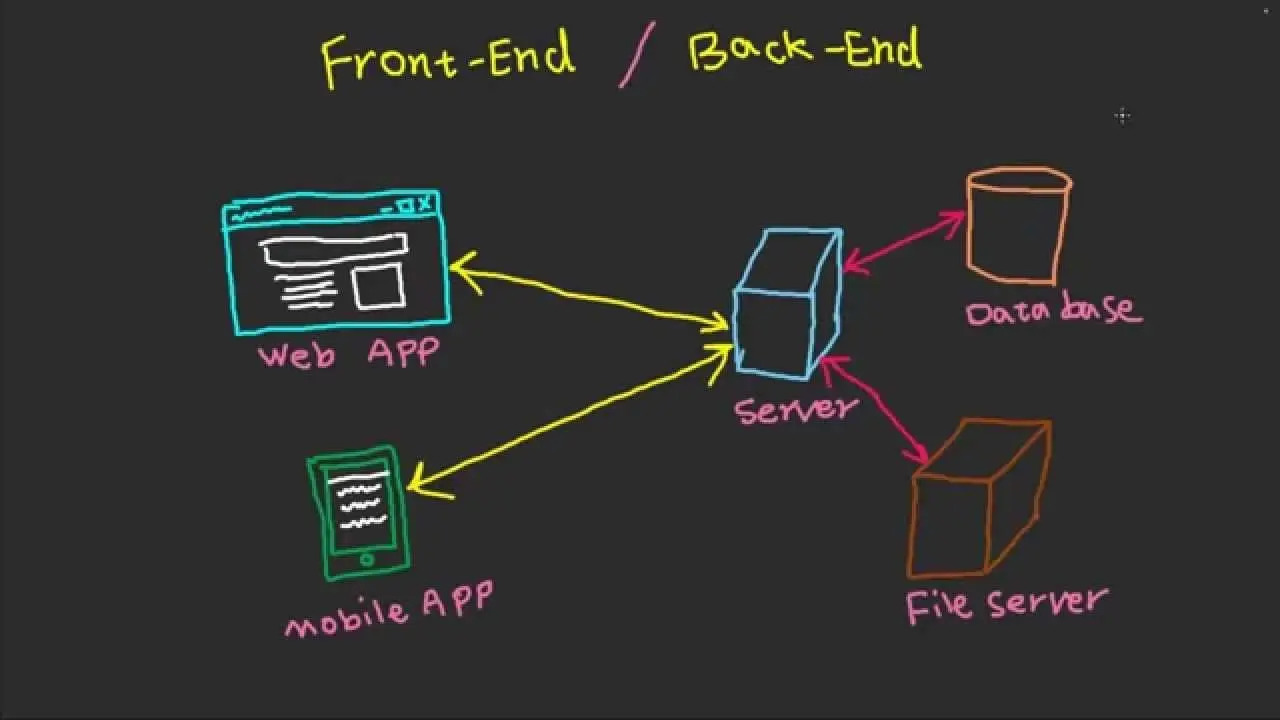
\includegraphics[width=10cm]{backend_database_relationship}
		\caption{A backend szerepe, forrás: \cite{backend}}
		\label{fig-backend}
	\end{figure}
	
	A backend tehát egy közvetítő szerepet tölt be a felhasználói felület és az adatbázis között. Emellett gondoskodik a rendszer biztonságáról is, például ellenőrzi, hogy ki férhet hozzá az adatokhoz, és biztosítja, hogy csak jogosult felhasználók kérhessenek vagy módosíthassanak információkat. Egy jól megtervezett backend képes kezelni a nagyszámú beérkező kérést, biztosítja az adatok gyors elérését, és ellenáll a különféle biztonsági fenyegetéseknek.
	
	A backend működését különböző programozási nyelvekkel lehet megvalósítani, például Node.js, Python vagy Java segítségével. Az adatfeldolgozási logikát általában szerveroldali alkalmazások biztosítják, amelyeket webes szervereken futtatnak. Ezek a szerverek fogadják a beérkező kéréseket, majd a megfelelő válaszokat küldik vissza a felhasználóknak.
	
	\section{Mi az adatbázis és hogyan tárolja az adatokat?}
	Az adatbázis a rendszer egyik legfontosabb komponense, hiszen itt tárolódnak a felhasználók személyes adatai, például a nevük, születési dátumuk és igazolványszámuk. Az adatbázisokat úgy tervezték, hogy az adatok gyorsan és hatékonyan lekérhetők, módosíthatók vagy törölhetők legyenek.
	
	A digitális személyi igazolványokat kezelő rendszerben az adatbázis nemcsak az igazolványok adatait tartalmazza, hanem azokhoz kapcsolódó egyéb információkat is, például a feltöltés időpontját vagy a kép elérhetőségét. Ezeket az adatokat táblázatos formában tárolják, ahol minden egyes rekord egy adott felhasználóhoz tartozik.
	
	Az adatbázisok különböző típusúak lehetnek. A relációs adatbázisok (pl. MySQL, PostgreSQL) táblázatos formában, előre definiált struktúrában tárolják az adatokat, míg a NoSQL adatbázisok (pl. MongoDB) rugalmasabb adatkezelést tesznek lehetővé, amely különösen előnyös lehet olyan alkalmazások számára, ahol az adatok struktúrája dinamikusan változhat.
	
	Az adatbázis hatékony működésének egyik alapfeltétele a megfelelő indexelés és optimalizáció, amely biztosítja, hogy a keresések gyorsan végrehajthatók legyenek, és a rendszer ne lassuljon le nagy mennyiségű adat esetén sem.
	\section{A backend és az adatbázis kapcsolata}
	A backend és az adatbázis folyamatos kommunikációban állnak egymással, és szorosan együttműködnek az adatok kezelésében. Amikor egy felhasználó kérést küld az alkalmazáson keresztül, például meg akarja tekinteni az igazolványa adatait, a backend továbbítja ezt a kérést az adatbázisnak. Az adatbázis ezután megkeresi a megfelelő információt, és visszaküldi azt a backendnek, amely feldolgozza az adatokat, majd elküldi a felhasználónak.
	
	A kapcsolat működését egy példán keresztül lehet a legjobban szemléltetni. Ha egy felhasználó bejelentkezik az alkalmazásba, és szeretné megtekinteni a személyi igazolványának adatait, akkor a következő lépések történnek:
	
	
	\begin{enumerate}
		\item 	A felhasználó kérést küld az alkalmazásban, hogy szeretné megtekinteni az igazolványát.
		\item 	A backend fogadja a kérést, és továbbítja az adatbázisnak.
		\item 	Az adatbázis megkeresi az adott felhasználóhoz tartozó igazolványadatokat, majd visszaküldi azokat a backendnek.
		\item 	A backend feldolgozza az adatokat, és továbbítja azokat a felhasználói felületre.
		\item 	A felhasználó az alkalmazás képernyőjén megkapja az igazolványa adatait.
	\end{enumerate}
	Ez a folyamat minden egyes adatlekérésnél vagy -módosításnál hasonló módon zajlik le.
	
	\section{Biztonság és adatvédelem}
	A digitális személyi igazolványokat kezelő rendszerek egyik legfontosabb kihívása az adatbiztonság és a személyes adatok védelme. Mivel ezek az adatok érzékeny információkat tartalmaznak, elengedhetetlen, hogy a backend és az adatbázis megfelelő védelmi intézkedésekkel legyen ellátva. A biztonsági kockázatok közé tartoznak a jogosulatlan hozzáférések, az adatszivárgások, valamint a kibertámadások, amelyek komoly következményekkel járhatnak.
	
	A személyes adatok védelme érdekében az egyik legfontosabb lépés az adattitkosítás. Az érzékeny információkat, például az igazolványszámokat és a felhasználói azonosítókat, titkosítva kell tárolni az adatbázisban, hogy még akkor se lehessen azokat közvetlenül elolvasni, ha valaki illetéktelen módon hozzáférne az adatokhoz. Az adattovábbítás során is elengedhetetlen a biztonság, ezért minden kommunikációnak titkosított csatornán, például HTTPS-en és TLS-protokollon keresztül kell történnie.
	
	A jogosultságkezelés egy másik kulcsfontosságú tényező, amely biztosítja, hogy az adatokhoz kizárólag az arra jogosult személyek vagy rendszerek férhessenek hozzá. A felhasználók azonosítása különböző módszerekkel történhet, például jelszavakkal, kétlépcsős hitelesítéssel vagy token-alapú megoldásokkal, mint amilyen a JWT (JSON Web Token). Emellett fontos, hogy a rendszerben szerepköröket és jogosultsági szinteket határozzunk meg, hogy egyes adatokhoz csak bizonyos felhasználók vagy adminisztrátorok férhessenek hozzá.
	
	Az adatvesztés és a rendszerleállások elkerülése érdekében elengedhetetlen a rendszeres biztonsági mentések készítése. Az adatok redundáns tárolása, például több szerveren vagy felhőalapú megoldásokon keresztül, biztosítja, hogy egy esetleges meghibásodás vagy támadás esetén is visszaállíthatók legyenek a kritikus információk. A biztonsági mentések mellett fontos a rendszeres auditálás és naplózás is, amely lehetővé teszi az esetleges visszaélések vagy jogosulatlan hozzáférések nyomon követését.
	
	A hálózati védelem ugyancsak kulcsfontosságú tényező a biztonság szempontjából. A szervereket és az adatbázisokat megfelelő tűzfalakkal és behatolásérzékelő rendszerekkel kell védeni a külső támadások ellen. Emellett az alkalmazásokat úgy kell megtervezni, hogy ellenálljanak az olyan gyakori támadásoknak, mint például az SQL injection vagy a Cross-Site Scripting (XSS). Az ilyen támadások megelőzése érdekében minden bemeneti adatot megfelelően ellenőrizni és szűrni kell, valamint a felhasználói adatokat biztonságosan kell kezelni.
	
	Összességében a backend és az adatbázis közötti szoros együttműködés biztosítja, hogy a digitális személyi igazolványok rendszere hatékonyan és biztonságosan működjön. A megfelelő technológiai megoldások alkalmazásával garantálható az adatok gyors elérhetősége, a stabil működés és a személyes adatok védelme, amely elengedhetetlen egy ilyen érzékeny adatokat kezelő alkalmazás esetében.
	
	\chapter{Frontend: Hogyan Találkozik a Felhasználó az Alkalmazással?}
	
	A frontend az alkalmazás azon része, amelyet a felhasználók közvetlenül látnak és használnak. Ez felelős az adatok megjelenítéséért, a felhasználói interakciók kezeléséért és az általános vizuális élmény biztosításáért. Ha a backend az étterem konyhája, ahol az ételek készülnek, akkor a frontend az étterem belső tere, ahol a vendégek leülnek, rendelnek és elfogyasztják az ételeiket. Az étlap, az asztalok elrendezése és a pincérek munkája mind a frontend részei ebben az analógiában.
	
	\section{A frontend szerepe a digitális rendszerekben}
	
	A frontend az a réteg, amely lehetővé teszi a felhasználók számára, hogy kapcsolatba lépjenek az alkalmazással. A digitális személyi igazolványokat kezelő alkalmazás esetében a frontend biztosítja, hogy a felhasználó egyszerűen és érthetően tudja elérni az igazolványának adatait, feltölteni egy új dokumentumot, vagy hitelesíteni magát a rendszerben.
	
	A frontend tehát egy közvetítő réteg a felhasználó és a háttérrendszer között. A felhasználó egy gomb megnyomásával utasítást adhat az alkalmazásnak, amely ezt a kérést továbbítja a backendhez. A backend feldolgozza a kérést, lekérdezi az adatbázisból az információt, és visszaküldi azt a frontendnek, amely megjeleníti azt a képernyőn.
	
	A frontend egyik legfontosabb feladata az intuitív és felhasználóbarát kezelőfelület biztosítása. Egy jól megtervezett felület könnyen érthető, logikusan felépített, és lehetővé teszi, hogy a felhasználó gyorsan elvégezze a kívánt műveleteket. Ha a frontend bonyolult vagy átláthatatlan, az akadályozhatja a rendszer használatát, és akár el is riaszthatja a felhasználókat.
	
	\section{A frontend technológiai alapjai}
	
	A frontend fejlesztése során olyan technológiákat alkalmaznak, amelyek lehetővé teszik a vizuális megjelenítést és a felhasználói interakciókat. Az egyik legelterjedtebb frontend nyelv a \textbf{HTML (HyperText Markup Language)}, amely az oldal szerkezetét határozza meg. A \textbf{CSS (Cascading Style Sheets)} segítségével a fejlesztők a dizájnt és a megjelenést szabályozzák, például a színek, betűtípusok és elrendezések beállításával. A \textbf{JavaScript} a frontend „motorja”, amely biztosítja az interaktivitást, például az űrlapok kitöltését, a gombokra való kattintás kezelését vagy az adatok valós idejű frissítését.
	
	Az egyszerű statikus weboldalak mellett a modern alkalmazások gyakran \textbf{dinamikus frontend keretrendszereket} használnak. Ilyen például a \textbf{React}, a \textbf{Vue.js} vagy az \textbf{Angular}, amelyek lehetővé teszik a komplex és interaktív kezelőfelületek létrehozását. A mobilalkalmazások esetében gyakran használják a \textbf{React Native} vagy a \textbf{Flutter} keretrendszereket, amelyekkel egyszerre lehet iOS és Android alkalmazásokat fejleszteni.
	
	\section{Hogyan működik a frontend és a backend együtt?}
	
	A frontend és a backend folyamatos kapcsolatban állnak egymással. Ha a felhasználó például beírja az alkalmazásba a felhasználónevét és jelszavát, majd megnyomja a „Bejelentkezés” gombot, akkor a frontend elküldi ezeket az adatokat a backendnek. A backend ellenőrzi az adatokat, és ha minden helyes, visszaküldi a megfelelő választ, amely alapján a frontend belépteti a felhasználót az alkalmazásba.
	
	A frontend és a backend közötti kommunikáció általában \textbf{API-kon (Application Programming Interface)} keresztül történik. Az API egyfajta közvetítő, amely meghatározza, hogy a két rendszer hogyan kommunikálhat egymással. A frontend egy API-hívást küldhet a backendnek, amely ezt feldolgozza, majd visszaküldi az eredményt a frontendnek.
	
	Egy digitális személyi igazolványokat kezelő alkalmazás esetében például egy API-hívás így nézhet ki:
	\begin{enumerate}
		\item A felhasználó feltölt egy személyi igazolványról készült képet a frontend felületén.
		\item A frontend elküldi ezt a képet a backendnek.
		\item A backend feldolgozza a képet egy OCR (optikai karakterfelismerő) rendszerrel, és kinyeri belőle az adatokat.
		\item A backend elmenti az adatokat az adatbázisba, majd visszaküldi a feldolgozott információkat a frontendnek.
		\item A frontend megjeleníti az adatokat a felhasználó számára egy könnyen olvasható formában.
	\end{enumerate}
	\section{A felhasználói élmény és a dizájn szerepe}
	
	Egy jól működő frontend nemcsak technológiailag fejlett, hanem vizuálisan is vonzó és könnyen használható. A \textbf{felhasználói élmény (UX – User Experience)} tervezése során a cél az, hogy az alkalmazás logikus és intuitív módon vezesse végig a felhasználót a szükséges lépéseken. Az \textbf{UI (User Interface)}, vagyis a felhasználói felület megtervezése szintén kulcsfontosságú, hiszen ez határozza meg az alkalmazás kinézetét és azt, hogy mennyire könnyű rajta eligazodni.
	
	Egy jó frontend dizájn figyelembe veszi a következőket:
	
	\begin{itemize}
		\item Az átlátható navigációt, hogy a felhasználók gyorsan megtalálják a szükséges funkciókat.
		
		\item Az egyszerű és logikus elrendezést, hogy az információk könnyen érthetőek legyenek.
		
		\item Az interaktív elemeket, amelyek visszajelzést adnak a felhasználónak, például egy gomb megnyomása után megjelenő betöltési animáció.
		
		\item A reszponzivitást, amely biztosítja, hogy az alkalmazás minden eszközön – mobilon, tableten és számítógépen is – megfelelően működjön.
	\end{itemize}
	
	\chapter{Backend fejlesztése Node.js segítségével}
	
A backend fejlesztés kulcsszerepet játszik a modern web- és mobilalkalmazások működésében, hiszen ezen a rétegen történik az adatok kezelése, tárolása és kiszolgálása. A szerveroldali technológiák közül a Node.js az egyik legnépszerűbb választás, amely lehetőséget biztosít arra, hogy az alkalmazás teljes fejlesztése JavaScript nyelven történjen. A Node.js egy gyors és hatékony futtatókörnyezet, amely eseményvezérelt és nem blokkoló működésének köszönhetően különösen alkalmas nagy teljesítményt igénylő alkalmazások készítésére.

\section{A Node.js alapjai és működési modellje}

A Node.js a Google V8 JavaScript motorjára épül, amely lehetővé teszi a JavaScript kód gyors végrehajtását szerveroldalon. Az egyik legfontosabb sajátossága az aszinkron és eseményvezérelt működés, amely lehetővé teszi, hogy a szerver egyszerre több kérést is kezeljen anélkül, hogy az egyes műveletek blokkolnák egymást. Mivel a Node.js nem használ többszálú feldolgozást, hanem egyetlen szálon fut, a skálázhatóságot egy úgynevezett eseményhurok biztosítja, amely a beérkező kéréseket folyamatosan fogadja és kezeli.

Az aszinkron működés egyik alapvető eszköze a visszahívási függvények (callback), amelyeket később az ígéretek (Promises) és az async/await konstrukciók egészítettek ki. Az alábbi példa bemutatja, hogyan lehet egy fájl beolvasását aszinkron módon végrehajtani a fs modul segítségével:

\lstinputlisting[style=myjavascript,caption=Egy Node.js kód,label=kod-nodejs1]{nodejs_1.js}

Ebben a kódrészletben a fájl beolvasása nem blokkolja a többi művelet végrehajtását, mivel az eredmény egy visszahívási függvényben kerül feldolgozásra. Ennek köszönhetően a szerver továbbra is képes új kérések kiszolgálására, miközben a fájl beolvasása háttérben történik.

\section{A Node.js előnyei és kihívásai}
A Node.js egyik legnagyobb előnye a teljesítménye és skálázhatósága. Az eseményvezérelt architektúra miatt a szerver könnyedén kezelhet nagy számú egyidejű kapcsolatot anélkül, hogy túlterhelődne. Ez különösen előnyös olyan alkalmazások esetében, amelyek valós idejű interakciót igényelnek, például csevegőalkalmazások vagy élő adatstreaming megoldások.

Egy másik fontos előny a JavaScript használata mind a frontend, mind a backend fejlesztés során. Ez lehetővé teszi, hogy a fejlesztőcsapatok egységes technológiai környezetben dolgozzanak, ami jelentősen csökkenti a fejlesztési időt és egyszerűsíti a kód karbantarthatóságát.

A Node.js azonban nem minden esetben ideális választás. A CPU-intenzív műveletek, például nagy mennyiségű számítási feladatokat végző algoritmusok vagy mesterséges intelligencia modellek futtatása esetén a Node.js teljesítménye korlátozott lehet. Mivel egyszálú környezetben működik, a nagy számítási igényű feladatok blokkolhatják az egész szerver működését. Ilyen esetekben érdemes külső szolgáltatásokat vagy külön szálakon futó háttérfolyamatokat használni a terhelés elosztására.

\section{Backend fejlesztés Express.js segítségével}

A Node.js önmagában is alkalmas szerverek létrehozására, de a fejlesztést jelentősen megkönnyíti az Express.js, amely egy minimalista és rugalmas webkeretrendszer. Az Express lehetőséget biztosít API végpontok kialakítására, HTTP kérések kezelésére és middleware-ek használatára.

Az alábbi példában egy egyszerű szerver hozható létre Express segítségével, amely egy alapvető GET végpontot biztosít:

\lstinputlisting[style=myjavascript,caption=Egy Node.js kód,label=kod-nodejs2]{nodejs_2.js}

Ez a kód mindössze néhány sorban egy működőképes HTTP szervert hoz létre, amely egy egyszerű üzenetet küld vissza a kliensek számára. Az Express egyik nagy előnye, hogy lehetővé teszi az útvonalak és middleware-ek könnyű kezelését, amelyek segítségével az alkalmazás bővíthető és testreszabható.

\section{Adatbázis-kezelés Node.js-ben}

A backend fejlesztés egyik alapvető feladata az adatkezelés, amelyhez különböző adatbázisokat lehet használni. A Node.js kompatibilis mind a relációs (SQL), mind a NoSQL adatbázisokkal. A relációs adatbázisok, például a MySQL vagy a PostgreSQL strukturált adatkezelést biztosítanak, míg a NoSQL megoldások, mint a MongoDB, rugalmasabb adatmodellezést tesznek lehetővé.

Egy MongoDB alapú adatbázis kapcsolat létrehozására a Mongoose csomag használható, amely egy objektumorientált adatmodellezést biztosító eszköz. Az alábbi példa egy egyszerű kapcsolat létrehozását és egy új adatrekord mentését mutatja be:

\lstinputlisting[style=myjavascript,caption=Egy Node.js kód,label=kod-nodejs3]{nodejs_3.js}

A Mongoose használata lehetővé teszi az adatbázis-interakciók egyszerű kezelését, miközben biztosítja az adatok validálását és strukturálását. Az objektumorientált modellnek köszönhetően a JavaScript objektumok könnyedén átalakíthatók adatbázis-bejegyzésekké.
	
\begin{thebibliography}{9}
	\bibitem{eIDAS} Európai Unió, \textit{Regulation (EU) No 910/2014 of the European Parliament and of the Council of 23 July 2014 on electronic identification and trust services for electronic transactions in the internal market}, Official Journal of the European Union, L 257/73, 2014.
	\bibitem{backend} \textsc{Mat Zaleski:} \textit{What Is a Mobile App Backend and Does Your Mobile Application Need It?}, 2024, \url{https://www.nomtek.com/blog/mobile-app-backend}
\end{thebibliography}
	
\end{document}